\documentclass{article}
\usepackage{xeCJK}
\usepackage{ctex}
\usepackage{listings}
\usepackage{xcolor, xparse}
\usepackage{setspace}
\usepackage{graphicx}
\usepackage[left=2.50cm, right=2.50cm, top=2.50cm, bottom=2.50cm]{geometry}
\usepackage{makecell}

\definecolor{mygreen}{rgb}{0,0.6,0}
\definecolor{mygray}{rgb}{0.5,0.5,0.5}
\definecolor{mymauve}{rgb}{0.58,0,0.82}
\definecolor{cmdbg}{rgb}{0.8,0.8,0.8}
\definecolor{shadecolor}{rgb}{0.92,0.92,0.92}

\lstset{
    language    = c++,
    numbers     = left,
    rulesepcolor= \color{gray},
    breaklines=true,
    % backgroundcolor=\color{cmdbg},
    numberstyle={
        \small
        \color{gray}
    },
    commentstyle = \color{gray},
    keywordstyle={
        \color[RGB]{175,0,175}
        \bfseries
    },
    stringstyle={
        \color[RGB]{0,125,0}
        \bfseries
    },
    basicstyle={
        \small\ttfamily
    },
    breaklines=true,
    tabsize     = 4,
    frame       = single,%主题
    columns     = fullflexible,
    rulesepcolor = \color{red!20!green!20!blue!20}, %设置边框的颜色
    showstringspaces = false, %不显示代码字符串中间的空格标记
    escapeinside={\%*}{*)},
}
\usepackage[CJKbookmarks=true]{hyperref}


\begin{document}

\pagestyle{empty}
%生成封面
\begin{figure}
    \centering
    
\includegraphics[width=0.35\textwidth]{xdu.jpeg}
\end{figure}

\begin{spacing}{4.0}
    \centering
    \textbf{\Huge 网络应用程序设计 \\ \LARGE 模拟FTP服务系统}
\end{spacing}

\begin{spacing}{2.5}
    \centering
    \Large 姓名: xxx \\ 学号:xxx  \\ 2021年6月29日
\end{spacing}
\newpage 

%生成目录
\setcounter{secnumdepth}{4} 
\setcounter{tocdepth}{4}  
\begin{spacing}{2.0}
    \tableofcontents
\end{spacing}
\newpage

%正文
\pagestyle{plain}
\setcounter{page}{1}
\begin{spacing}{2.0}
\section{实验内容}
    本次实验中,我们在真实的网络环境下搭建安全的文件传输系统,使得客户端与服务器之间能够进行任意类型文件的安全传输。
\section{实验环境}
    客户机使用Ubuntu 20.04.2 LTS操作系统,服务器使用Ubuntu 18.04.5 LTS操作系统。
\section{内容分析}
    考虑到文件传输需要高可靠性,本次实验中我们使用\textbf{socket/tcp}完成数据传输。

    双方首先通过socket套接字建立连接,随后通过对称密钥分发办法(如DH、Elgalma等)分享会话密钥,此后的即可使用该密钥对文件进行加解密。

    服务器支持如下四种操作:
    \begin{spacing}{1.5} \begin{itemize}
        \item 列出当前目录下所有文件的详细信息
        \item 删除当前目录下某个文件
        \item 上传某文件到服务器
        \item 下载某文件到客户端
    \end{itemize} \end{spacing}
\section{具体实现}
    \subsection{文件清单}
        下面给出所有文件及文件夹的说明。
    \begin{lstlisting}
Makefile: makefile文件
rqdmap.h: 个人编程时惯用的一些宏定义
ftp.h, ftp.cpp: 定义了一些便于SOCKET通讯的结构体、函数等
des/: 文件夹内包含了DES实现的源码
run_des.o: 封装了DES加解密的接口
server.cpp, server: 服务器源码及主程序
client.cpp, client: 客户端源码及主程序
pic.gif: 测试用例,检验图片是否能完好的传输
    \end{lstlisting}

    \subsection{准备工作}   
        \subsubsection{TCP消息的读取}
            TCP是面向字节流的协议,因而在接下来的设计中我们大量使用
            \begin{center}
                \fcolorbox{black}{shadecolor}{\{报文类型, 32位整数N, N字节数据流\}}
            \end{center}
            的形式来传输数据。
            而实际网络中存在各种情况,因而有可能存在这样的情形:消息接收方一次读取消息后得到了即将应该接收的字节数N,但是暂时只收集到了不足n的字节流,此时接收方应该不断循环读取,直到读到的字节数不小于N才停止。
            为此,我们实现了一个基于\textbf{循环队列}的消息队列,用于不断地读取消息,并能反馈出目前读取字节的长度。下面给出该消息队列的接口信息:
            \lstinputlisting[firstline = 23, lastline=35]{../ftp/ftp.h}

        \subsubsection{密钥分发算法}
            这里我们使用DH算法分发对称加密密钥,为此需要实现快速幂算法来进行$O(logN)$幂次计算。接口信息如下:
            \lstinputlisting[firstline = 37, lastline=38]{../ftp/ftp.h}
        \subsubsection{加解密算法}
            考虑到本次实验仅仅是对安全FTP系统的一次简单模拟,故使用较为简单的DES作为对称加密算法以说明原理。
            加解密算法单独成为一套接口\fcolorbox{black}{shadecolor}{run\_des.o},可以通过如下方式进行调用:
        \begin{lstlisting}
./run_des.o -g <OutKeyFile>           //产生密钥,存放在OutKeyFile中
./run_des.o -e <KeyFile> <From> <To>  //使用KeyFile加密From文件,产出到To中
./run_des.o -d <KeyFile> <From> <To>  //使用KeyFile解密From文件,产出到To中
        \end{lstlisting}

    \subsection{FTP功能}
    FTP功能一共有四个: \textbf{列出所有可访问文件、删除文件、上传文件、下载文件}, 下面将逐一进行说明。

    首先给出通讯过程中用到的功能关键字的宏定义:
    \lstinputlisting[firstline=10, lastline=17]{../ftp/ftp.h}

    \subsubsection{列出所有可访问文件} 客户端首先发送功能关键字LIST进行请求,服务器端接到后使用系统调用\fcolorbox{black}{shadecolor}{system(``ls -al")},读取调用结果,并将结果返回给客户端。
    客户端根据数据流的格式解析出数据内容,将结果显示在控制台。
    
    双方通讯中字节流的交互流程如下所示:
    
    \indent \indent Client 发送: \fcolorbox{black}{shadecolor}{LIST} 

    \indent \indent Server 发送: \fcolorbox{black}{shadecolor}{CONTENT + \{数据内容\} + FIN} 

    \indent \indent Client 本地显示数据内容

    \subsubsection{删除文件} 客户端发送功能关键字DELETE和想要删除的文件名给服务器,服务器接收到后首先进行合法性检验,确保用户删除的文\textbf{存在}且不得超出当前文件夹范围,随后再进行文件删除,返回状态给客户。

    双方通讯中字节流的交互流程如下所示:

    \indent \indent Client: \fcolorbox{black}{shadecolor}{DELETE + \{文件名\}} 

    \indent \indent Server: \fcolorbox{black}{shadecolor}{ACK/NAK} 

    ACK表示删除成功,NAK表示删除失败。

    \subsubsection{上传文件} 客户端发送功能关键字UPLOAD和想要上传的文件名及其大小,服务端进行文件创建并开辟空间,随后客户端再传输具体的字节流,服务端接受字节流并写入文件。

    双方通讯中字节流的交互流程如下所示:

    \indent \indent Client 发送: \fcolorbox{black}{shadecolor}{UPLOAD \{文件名\} }

    \indent \indent Server 在本地创建该文件,并反馈: \fcolorbox{black}{shadecolor}{ACK/NAK}

    \indent \indent 如果接收到\fcolorbox{black}{shadecolor}{ACK}, Client 发送: \fcolorbox{black}{shadecolor}{\{文件大小\} }

    \indent \indent Server 在本地为该文件开辟空间,并反馈: \fcolorbox{black}{shadecolor}{ACK/NAK}

    \indent \indent 如果接收到\fcolorbox{black}{shadecolor}{ACK}, Client 加密原始文件,发送: \fcolorbox{black}{shadecolor}{\{密文文件数据流\} + FIN}

    \indent \indent Server 不断读密文数据并保存到文件中,解密密文文件,如果成功则反馈: \fcolorbox{black}{shadecolor}{ACK}

    \indent \indent Client 接收: \fcolorbox{black}{shadecolor}{ACK}, 认为文件传输成功。

    \subsubsection{下载文件} 下载文件与上传文件类似。客户发送想要下载的文件名,服务端检查该文件是否存在,如果存在,则使用与\textbf{上传文件}类似的交互方式完成文件传输,便不予赘述。
        
\section{结果展示}
    运行两个程序(\textit{client, server}),双方连接成功,交换密钥成功。
\begin{center}
    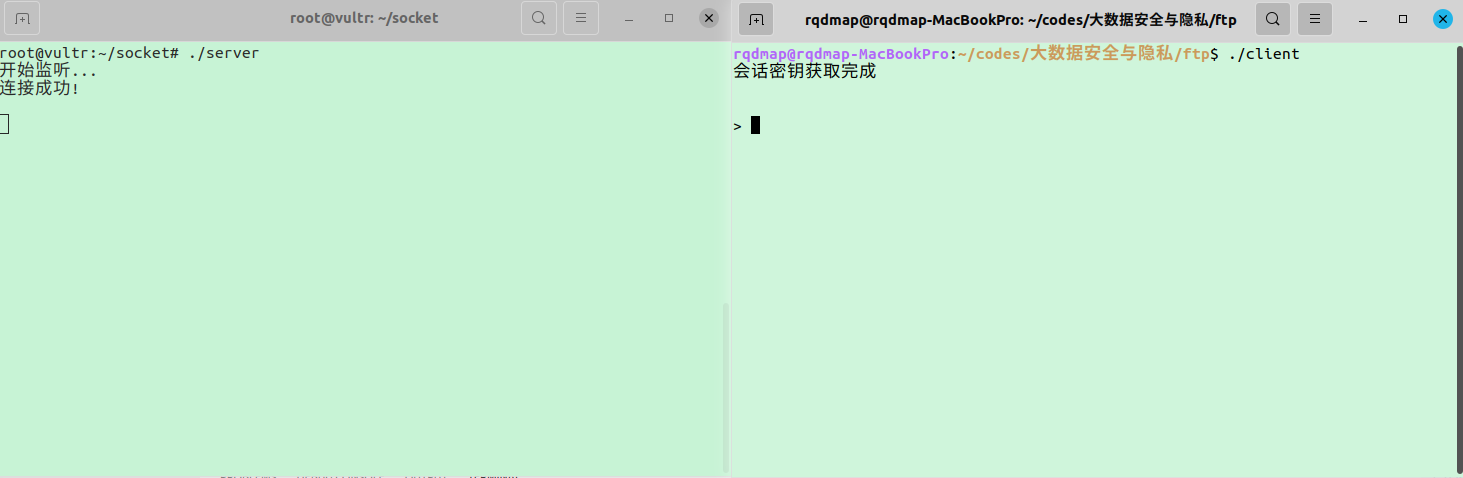
\includegraphics[width=1\textwidth]{pic/1.png}
\end{center} 

    客户端使用\textit{ls}指令查看服务器上所有可供访问的资源。

\begin{center}
    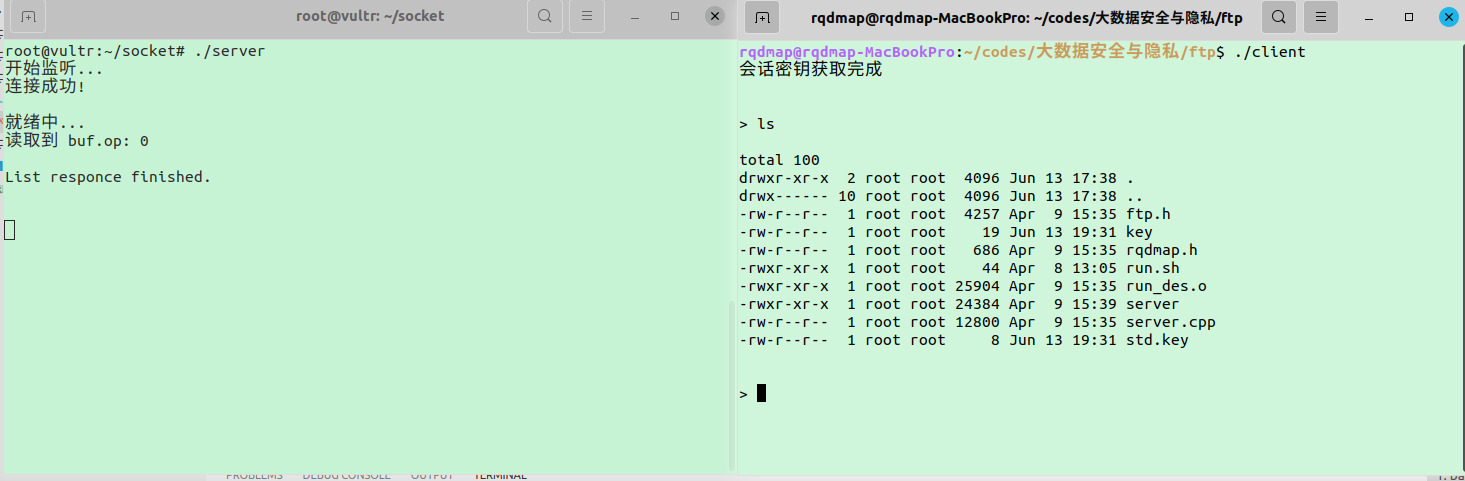
\includegraphics[width=1\textwidth]{pic/2.png}
\end{center} 

    客户端上传本地的一张图片\textit{pic.gif}, 上传完成后显示花费时间。
\begin{center}
    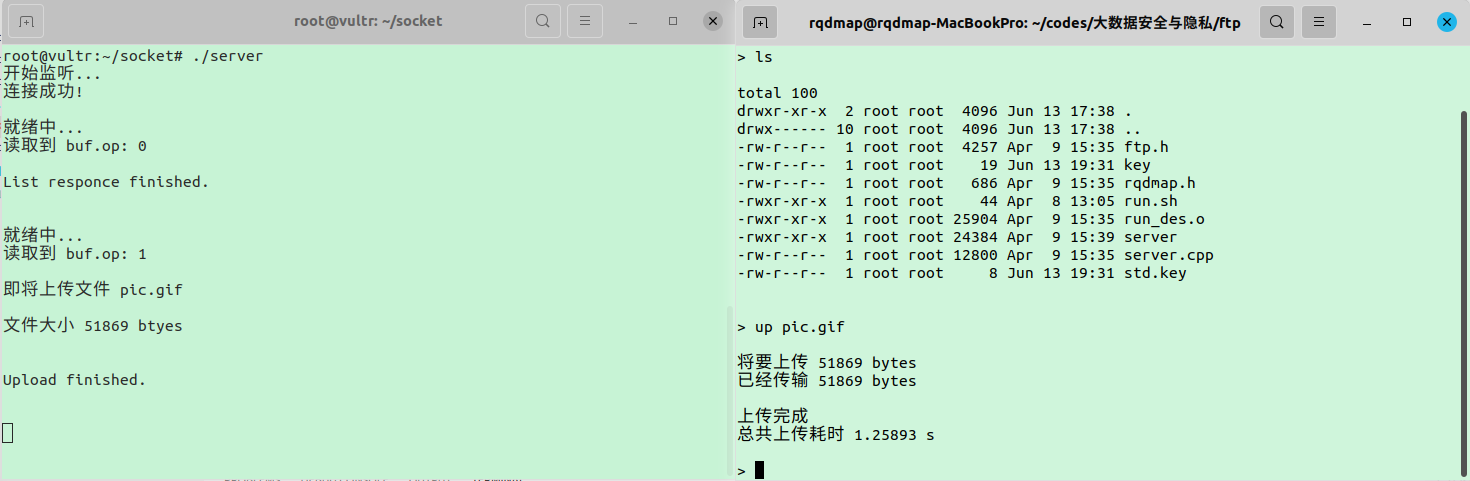
\includegraphics[width=1\textwidth]{pic/3.png}
\end{center} 

    客户端使用\textit{ls}指令检查是否成功上传图片,并使用\textit{rm}指令删除该图片。

\begin{center}
    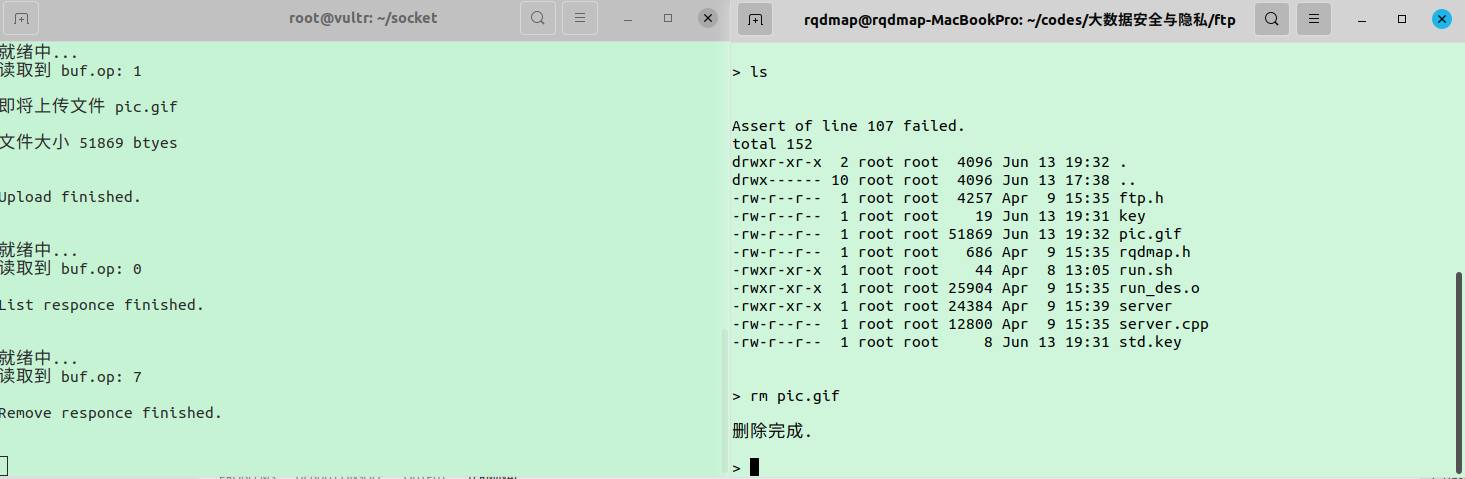
\includegraphics[width=1\textwidth]{pic/4.png}
\end{center}
\section{局限与展望}
\begin{spacing}{1.5} \begin{itemize}
    \item FTP服务器暂时不支持文件夹操作
    \item 不同用户之间没有进行认证与分类,全部共用一套公用的文件夹
    \item 加密算法基于文件而不是对字节流进行加密,会导致部分操作码的明文泄漏,有一定的安全问题
    \item 尚未实现多用户功能。由于多用户涉及到消息队列的异步读取、父子进程的协调工作等,本次实验时间较紧,故暂不支持多用户系统。
\end{itemize} \end{spacing}

\end{spacing}
\end{document}